\section{Спин--орбитальное взаимодейтвие в приближении сильной связи}
Необходимым ``ингредиентом'' для топологических изоляторов является спин--орбитальное 
взаимодействие. Экспериментальная реализация \cite{Bernevig2006, Konig2007} двумерного топологического изолятора ---
квантовая яма CdTe--HgTe--CdTe, составляющие которой --- узкозонные полупроводники с 
сильным спин--орбитальным расщеплением. Для их описания давно применяются
гамильтонианы Латтинжера и Кейна (\cite{Luttinger1956,Kane1957}). Однако эти гамильтонианы
выводятся из симметрийных соображений в $k\cdot p$ методе и, следовательно,
дают спектр только в центре зоны Бриллюэна, а также не слишком интуитивно понятны.

Мы построили простую модель сильной связи, аналогичную модели Кейна, 
учитывающую валентную $p$--зону и $s$--зону проводимости. Как показано, она переходит
в модель Кейна при малых $k$. Также она даёт возможность найти спектр во всей зоне 
Бриллюэна, а также интуитивно понятным образом описать одиночные примеси, границы образца,
резкие изменения параметров и прочее.

Модель представляет из себя 
кубическую решётку из атомов, на каждом из которых ``сидят'' состояния
с $p_x$--, $p_y$--, $p_z$-- и $s$--орбиталями и двумя 
возможными проекцими спина. В модели учитывались перекрытия
орбиталей соседних атомов, а также внутриатомное спин--орбитальное взаимодействие.
В литературе утверждается, что эффекты от межатомного спин--орбитального 
взаимодействия пренебрежимо малы.

Для написания
спин--орбитального гамильтониана $p$--зоны необходимо перейти к состояниям с определённым
полным моментом. Эти состояния выражаются через $p_x$, $p_y$, $p_z$ орбитали следующим образом:
\begin{equation}
	\label{transform1}
	\begin{gathered}
        \Psi_{\frac{3}{2},\frac{3}{2}} = \frac{X + iY}{\sqrt{2}}\alpha\\
        \Psi_{\frac{3}{2}, \frac{1}{2}} = \sqrt{\frac{1}{3}}\frac{X + iY}{\sqrt{2}}\beta -
                                         \sqrt{\frac{2}{3}} Z\alpha\\
        \Psi_{\frac{3}{2}, -\frac{1}{2}} = -\sqrt{\frac{1}{3}}\frac{X - iY}{\sqrt{2}}\alpha -
                                         \sqrt{\frac{2}{3}} Z\beta\\
        \Psi_{\frac{3}{2},-\frac{3}{2}} = -\frac{X - iY}{\sqrt{2}}\beta
	\end{gathered}
\end{equation}
\begin{equation}
	\label{transform2}
	\begin{gathered}
        \Psi_{\frac{1}{2}, \frac{1}{2}} = \sqrt{\frac{2}{3}}\frac{X + iY}{\sqrt{2}}\beta +
                                         \sqrt{\frac{1}{3}} Z\alpha\\
        \Psi_{\frac{1}{2}, -\frac{1}{2}} = -\sqrt{\frac{2}{3}}\frac{X - iY}{\sqrt{2}}\alpha-
                                         \sqrt{\frac{1}{3}} Z\beta\\
	\end{gathered}
\end{equation}
Здесь $X,Y,Z$ --- атомные орбитали, $\alpha,\beta$ --- состояния со спином вверх и вниз.

Как хорошо известно, в атоме гамильтониан спин--орбитального взаимодейстия имеет вид
\begin{equation}
    H_{\mathrm{SO}} =  A(\vec{S}, \vec{L}) = \frac{A}{2}(J^2 - L^2 - S^2)
\end{equation}
Если орбитальный момент фиксирован, то энергия определяется полным моментом. Таким образом,
спин--орбитальное взаимодействие приводит к расщеплению состояний с моментами $\frac32$ и
$\frac12$.

Пусть матричные элементы перекрытия $p$-- орбиталей --- $t_\parallel$ и $t_\perp$. Тогда
несложно показать, что гамильтониан тяжёлых и лёгких дырок в импульсном представлении ---
\begin{equation}
    \begin{gathered}
    H_v = \begin{bmatrix}
            H_l & H_r
        \end{bmatrix},\\
    H_l = 
    \begin{pmatrix}
        (t_\parallel + t_\perp)(\cos{p_x} + \cos{p_y}) + 2t_\perp \cos{p_z} & 0 \\
        0 & \left(\frac{t_\parallel}{3} + \frac{5t_\perp}{3}\right)(\cos{p_x}+\cos{p_y})+ 
                           \left(\frac{2t_\perp}{3} + \frac{4t_\parallel}{3}\right)\cos{p_z} \\
        -\frac{1}{\sqrt{3}}(t_\parallel - t_\perp)(\cos{p_x} - \cos_{p_y}) & 0 \\
        0 & -\frac{1}{\sqrt{3}}(t_\parallel - t_\perp)(\cos{p_x} - \cos_{p_y}) 
    \end{pmatrix}\\
    H_r = 
    \begin{pmatrix}
        -\frac{1}{\sqrt{3}}(t_\parallel - t_\perp)(\cos{p_x} - \cos_{p_y}) & 0 \\
        0 & -\frac{1}{\sqrt{3}}(t_\parallel - t_\perp)(\cos{p_x} - \cos_{p_y})\\
       \left(\frac{t_\parallel}{3} + \frac{5t_\perp}{3}\right)(\cos{p_x} + \cos{p_y}) + 
                    \left(\frac{2t_\perp}{3} + \frac{4t_\parallel}{3}\right)\cos{p_z} & 0 \\
        0 & (t_\parallel + t_\perp)(\cos{p_x} + \cos{p_y}) + 2t_\perp \cos{p_z}
    \end{pmatrix}
    \end{gathered}
\end{equation}
Эту матрицу можно разложить около нуля. Тогда получится хорошо известный 
гамильтониан Латтинжера \cite{Luttinger1956}:
\begin{equation}
    H_v = -\left(\gamma_1 + \frac{5}{2}\gamma_2\right) k^2 + 
        2\gamma_2(k_x^2J_x^2 + k_y^2J_y^2 + k_z^2J_z^2),
\end{equation}
где $J_i$ --- операторы момента для спина $\frac{3}{2}$, $\gamma_1 = \frac13 t_\parallel$,
$\gamma_2 = \frac16(t_\parallel - t_\perp)$, $\gamma_3 = 0$ (последнее слагаемое 
из гамильтониана Латтинжера опущено).

Теперь учтём перекрытие с $s$--зоной. Оно задаётся матрицей
\begin{equation}
    T = P\begin{pmatrix}
            -\frac{1}{\sqrt{2}}(\sin{p_x} + i\sin{p_y}) & \sqrt{\frac{2}{3}}\sin{p_z} &
             \frac{1}{\sqrt{6}}(\sin{p_x} - i\sin{p_y}) & 0 \\  
            0 & -\frac{1}{\sqrt{6}}(\sin{p_x} + i\sin{p_y}) & 
            \sqrt{\frac{2}{3}}\sin{p_z} & \frac{1}{\sqrt{2}}(\sin{p_x} - i\sin{p_y}),
         \end{pmatrix},
\end{equation}
где $P = 2i\langle s(x+e_x) | \hat{H} | p_x(x)\rangle$. Наконец, гамильтониан самой 
$s$--зоны можно записать как 
\begin{equation}
    H_c = (E_s + \frac{1}{m_s}(3 - \cos{p_x} - \cos{p_y} - \cos{p_z}))I_{2\times2}
\end{equation}
Состояниями с полным моментом $\frac{1}{2}$ 
можно пренебречь, если спин--орбитальное взаимодейтвие велико.
Таким образом мы получаем гамильтониан с учётом $s$--зоны проводимости, зон тяжёлых и
лёгких дырок в виде
\begin{equation}
    \label{hfull}
    H_{\mathrm{full}} = \begin{pmatrix}
                            H_c & T \\
                            T^\dagger & H_v
                        \end{pmatrix},
\end{equation}
где $H_c, T, H_v$ определены выше. Линеаризуя его, мы получим гамильтониан модели Кейна
\cite{Kane1957}.

Спектр такой модели не может быть найден аналитически для произвольных $k_x, k_y, k_z$. Однако
ветви спектра можно легко найти, если, например, $k_x = k_y = 0$. Для этого случая 
спектр в окрестности центра зоны Бриллюэна изображён на рисунке. Как видно, он состоит
из трёх ветвей: одной электронной ветви и двух ветвей дырок, тяжёлых и лёгких.

\begin{figure}
    \centering
    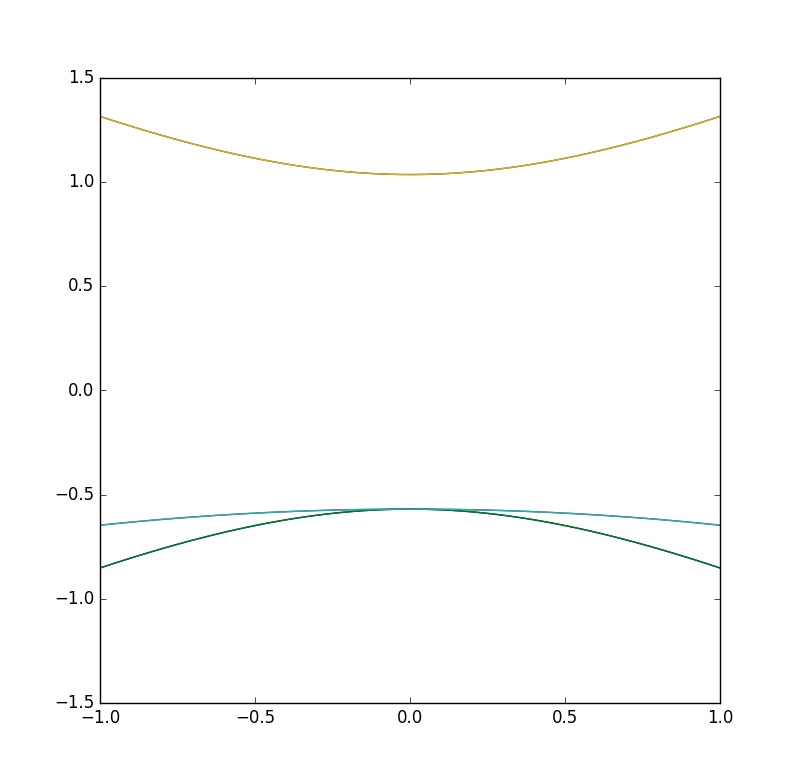
\includegraphics[width=0.6\linewidth]{cdte.png}
    \caption{На графике изображены ветви спектра CdTe в модели Кейна для параметров
             из \cite{Novik2005}. По оси абсцисс отложен волновой вектор в $\mathrm{nm}^{-1}$,
             по оси орбинат --- энергия в eV.}
\end{figure}

Таким образом, простая модель сильной связи воспроизводит известные свойства 
полупроводников со спин--орбитальным взаимодействием.

%\begin{equation}
%\scalebox{0.6}{%
%$
%H_v = \begin{pmatrix}
%       (t_\parallel + t_\perp)(\cos{p_x} + \cos{p_y}) + 2t\perp \cos{p_z} & 0 &
%       -\frac{1}{\sqrt{3}}(t_\parallel - t_\perp)(\cos{p_x} - \cos_{p_y}) & 0 \\
%
%       0 & \left(\frac{t_\parallel}{3} + \frac{5t_\perp}{3}\right)(\cos{p_x} + \cos{p_y}) + 
%                   \left(\frac{2t_\perp}{3} + \frac{4t_\parallel}{3}\right)\cos{p_z} & 
%       0 & -\frac{1}{\sqrt{3}}(t_\parallel - t_\perp)(\cos{p_x} - \cos_{p_y})\\
%       -\frac{1}{\sqrt{3}}(t_\parallel - t_\perp)(\cos{p_x} - \cos_{p_y}) & 0 &
%      \left(\frac{t_\parallel}{3} + \frac{5t_\perp}{3}\right)(\cos{p_x} + \cos{p_y}) + 
%                   \left(\frac{2t_\perp}{3} + \frac{4t_\parallel}{3}\right)\cos{p_z} & 0 \\
%       0 & -\frac{1}{\sqrt{3}}(t_\parallel - t_\perp)(\cos{p_x} - \cos_{p_y}) & 
%       0 & (t_\parallel + t_\perp)(\cos{p_x} + \cos{p_y}) + 2t\perp \cos{p_z}
%      \end{pmatrix}
%$
%}
%\end{equation}


%Гамильтониан имеет вид
%\begin{multline}
%   \label{well_model_ham}
%   H  = \sum_{m,n} (E_s + 4t_s) s_{mn}^{\dagger} s_{mn} - t_s s_{mn}^{\dagger}
%                          (s_{m+1,n} + s_{m-1,n} + s_{m,n+1} + s_{m,n-1}) \\
%          + t_{sp} s_{mn}^{\dagger} (-p_{m+1,n}^x + p_{m-1,n}^x - p^y_{m,n+1} + p^y_{m,n-1})
%                                                                + \mathrm{h.c.}  \\
%          + (p_{mn}^x)^{\dagger}(t_{\parallel}(p_{m+1,n}^x + p_{m-1,n}^x) +
%                                 t_{\perp} (p^x_{m,n+1} + p^x_{m,n-1})) \\
%          + (p_{mn}^x)^{\dagger}(t_{\perp}(p_{m+1,n}^y + p_{m-1,n}^y) +
%                                 t_{\parallel} (p^y_{m,n+1} + p^y_{m,n-1})) \\
%          + (p_{mn}^z)^{\dagger} t_3 (p_{m+1,n}^z + p_{m-1,n}^z +
%                                p^z_{m,n+1} + p^z_{m,n-1}) \\
%          -\frac{E_{SO}}{3}
%                \begin{matrix}
%                    \left(\begin{matrix}
%                        p_x^\dagger & p_y^\dagger & p_z^\dagger
%                    \end{matrix}\right) \\
%                    \\
%                    \\
%                \end{matrix}
%        		\left(\begin{matrix}
%        			1 & i & -1 \\
%        			-i & 1 & i \\
%        			-1 & -i & 1
%        		\end{matrix} \right)
%                \left(\begin{matrix}
%                    p_x \\ 
%                    p_y \\
%                    p_z
%                \end{matrix}\right) + \\
%        + \text{всё то же самое с переворотом проекции спина}
%\end{multline}
%
%Тогда спин--орбитальный гамильтониан запишется так:
%\begin{equation}
%	H_{\mathrm{full}} = -\Delta E_{SO} 
%			(a_{\frac{1}{2}, \frac{1}{2}}^\dagger a_{\frac{1}{2}, \frac{1}{2}} +
%			a_{\frac{1}{2}, -\frac{1}{2}}^\dagger a_{\frac{1}{2}, -\frac{1}{2}})
%\end{equation}
%После простого преобразования получается последнее слагаемое в \eqref{well_model_ham}.
